%% Example of a document

This example document aims to provide some examples of what \LaTeX{} can do.
For more examples, see \citetitle{wikibook-latex} \cite{wikibook-latex}.
Another good tutorial is \url{http://www.andy-roberts.net/misc/latex/}.

\section{Simple text}

Paragraphs are simply written as text.
Line returns and spacing in general do not matter for the formatting of the
document.

A new paragraph starts after leaving a blank line. \\
A line return is made using \lstinline$\\$.

All the commands are preceded by a \textbackslash{}, and their options are
between brackets \{ and \}.
% This is a comment
These can be preceded by "optional" options which are in square brackets [ and
].
So, \lstinline$\textbackslash{}$ produces a \textbackslash{}.
You can also use \textbackslash{} to escape some characters.
If you forget to put braces, spaces after the command name will be ignored

Comments start after a \% character.
If a line ends with a comment, the line return is also commented and is not
considered by latex.

Splitting the source across several files gives you more control, so to include
a file you use \lstinline$\documentclass[a4paper
	,11pt
	%,landscape
	%,openright
	%,twocolumn
	%,twoside
	]{article}
	%]{report}
\usepackage[utf8]{inputenc}

%% Meta-information
\def\doclanguage{}
\def\docauthor{[AUTHOR]}
\def\doctitle{[TITLE]}
\def\docdate{\today}
\def\docsubject{}
\def\dockeywords{}
\def\doctitlepagename{}
\def\docorganization{}
\def\doclogo{}
\def\doctocdepth{2}
% For the title page
\author{\docauthor}
\title{\doctitle}
\date{\docdate}
\def\docabstract{}

%% Style
%% document-style

%% common-document

\input{input/common}

%% Packages
\usepackage[pdftex]{hyperref}
\usepackage[pdftex]{graphicx} % Include graphics
\usepackage{grffile} % File names fix (graphicsx '.' in names)
\usepackage{tabularx} % Tables (extended)
\usepackage{float} % Floats (extended)
\usepackage{wrapfig} % Wrapping text around figures
\usepackage[table]{xcolor} % Colors
\usepackage{multirow} % Row spanning in tables

\usepackage{fancyhdr} % Headers and footers
\usepackage{lastpage} % \pageref{LastPage} % Must be compiled 2 times!
\usepackage{acronym} % For acronyms
\usepackage{makeidx} % Index
\usepackage{setspace} % Changing the interline
\usepackage{rotating} % Rotated text

%% Code formatting
\input{input/listings}

%% TikZ (drawing)
\input{input/tikz}

%% Bibliography
\usepackage[natbib=false
	%,sorting=none
	]{biblatex}

%% Macros
\input{input/macros}


%% Hypertext, links
\hypersetup{pdftex
	,pdfauthor={\docauthor}
	,pdftitle={\doctitle}
	,pdfsubject={\docsubject}
	,pdfkeywords=\dockeywords
	,colorlinks=true
	,linkcolor=black
	,urlcolor=blue
	,citecolor=teal
	,filecolor=magenta
	}

%% Code formatting
\lstset{%
%	,frame=single
%	,numbers=left
	,numberstyle=\tiny
	,numbersep=5pt
	,stepnumber=5
}

%% Options and lengths
%\setlength{\parindent}{0cm} % paragraphs indentation
%\parskip=5pt % distance between paragraphs
%\linespread{1.5} % interline distance
%\renewcommand{\labelitemi}{$\bullet$}
%\numberwithin{equation}{section}

%% Margins
\usepackage{a4wide}
%\addtolength{\textheight}{+2cm}
%\addtolength{\topmargin}{-1cm}
%\addtolength{\oddsidemargin}{-1cm}
%\addtolength{\textwidth}{+2cm}

%% Page style
\pagestyle{fancy}
%\pagestyle{empty}


%% Bilbiography and indexes
\bibliography{biblio}
\makeindex

%%%%%%%%%%%%
% Document %
%%%%%%%%%%%%
\begin{document}

%%%%%%%%%%%%%%%%%
% Title section %
%%%%%%%%%%%%%%%%%
%% document-begin
%% (title page and toc)

\ifthenelse{\equal{\doctitlepagename}{}}{
\maketitle
}{
\input{input/title/title_\doctitlepagename}
}

\ifthenelse{\equal{\docabstract}{}}{}{
\begin{abstract}
\docabstract
\end{abstract}
}
%\vspace*{\fill}
%\clearpage

%% Headers and footers
\lhead{}
\chead{}
\rhead{\bfseries \doctitle}
\lfoot{\docauthor}
\cfoot{}
\rfoot{\langOF{\thepage{}}{\pageref{LastPage}}}

%% TOC
\tableofcontents
\ifthenelse{\equal{\doctitlepagename}{}}{
\vspace*{\fill}
}{
\clearpage
}


%%%%%%%%%%%%%
% Body text %
%%%%%%%%%%%%%

%% Example of a document

This example document aims to provide some examples of what \LaTeX{} can do.
For more examples, see \citetitle{wikibook-latex} \cite{wikibook-latex}.
Another good tutorial is \url{http://www.andy-roberts.net/misc/latex/}.

\section{Simple text}

Paragraphs are simply written as text.
Line returns and spacing in general do not matter for the formatting of the
document.

A new paragraph starts after leaving a blank line. \\
A line return is made using \lstinline$\\$.

All the commands are preceded by a \textbackslash{}, and their options are
between brackets \{ and \}.
% This is a comment
These can be preceded by "optional" options which are in square brackets [ and
].
So, \lstinline$\textbackslash{}$ produces a \textbackslash{}.
You can also use \textbackslash{} to escape some characters.
If you forget to put braces, spaces after the command name will be ignored

Comments start after a \% character.
If a line ends with a comment, the line return is also commented and is not
considered by latex.

Splitting the source across several files gives you more control, so to include
a file you use \lstinline$\documentclass[a4paper
	,11pt
	%,landscape
	%,openright
	%,twocolumn
	%,twoside
	]{article}
	%]{report}
\usepackage[utf8]{inputenc}

%% Meta-information
\def\doclanguage{}
\def\docauthor{[AUTHOR]}
\def\doctitle{[TITLE]}
\def\docdate{\today}
\def\docsubject{}
\def\dockeywords{}
\def\doctitlepagename{}
\def\docorganization{}
\def\doclogo{}
\def\doctocdepth{2}
% For the title page
\author{\docauthor}
\title{\doctitle}
\date{\docdate}
\def\docabstract{}

%% Style
\input{input/document-style}

%% Bilbiography and indexes
\bibliography{biblio}
\makeindex

%%%%%%%%%%%%
% Document %
%%%%%%%%%%%%
\begin{document}

%%%%%%%%%%%%%%%%%
% Title section %
%%%%%%%%%%%%%%%%%
\input{input/document-begin}

%%%%%%%%%%%%%
% Body text %
%%%%%%%%%%%%%

\input{document-example}

\vspace*{\fill}
%%%%%%%%%%
% Ending %
%%%%%%%%%%
%\clearpage

%% Bibliography, indexes and lists
%\listoffigures
%\listoftables
%\nocite{*} % include all citations
\printbibliography
\printindex
\vspace*{\fill}

%%%%%%%%%%%%
% Appendix %
%%%%%%%%%%%%
\appendix

%\input{appendix}

\end{document}
$.
In \LaTeX{} you don't need to specify the extension of included files.

\subsection{Environments}

You can create lists, enumerations, ...

\begin{itemize}
\item itemize
\item nested
	\begin{itemize}
	\item n
	\end{itemize}
\end{itemize}

\begin{enumerate}
\item enumerate
\item nested
	\begin{enumerate}
	\item n
	\end{enumerate}
\end{enumerate}

\begin{description}
\item[a] \emph{description}.
\item[b] something else
\end{description}

\begin{quote}
A simple quote.
\end{quote}

\begin{quotation}
A longer quotation.
\end{quotation}

\subsection{Text formatting}

\paragraph{Size}
You can change the size: {\tiny tiny}, {\scriptsize scriptsize}, {\footnotesize
footnotesize}, {\small small}, {\normalsize normal}, {\large large}, {\Large
Large}, {\LARGE LARGE}, {\huge huge} or {\Huge Huge}.

\paragraph{Font family}
You can use either \lstinline${\_family text}$ or \lstinline$\text_{text}$ where
\_ is: \textrm{rm}, \textsf{sf}, \texttt{tt}.

\paragraph{Series, shapes and related}
\begin{itemize}
\item \emph{emphasis}
\item {\bfseries bfseries} bold
\item {\mdseries mdseries} medium
\item {\upshape upshape} normal shape
\item {\itshape itshape} italic
\item {\scshape scshape} small capitals
\item {\slshape slshape} slanted \pcomment{oblique}
\end{itemize}

\paragraph{Colors}
The \texttt{xcolor} package allows you to write {\color{red} in red}.

\paragraph{Case-changing}
\uppercase{UpperCase \pagename}, \lowercase{LowerCase \pagename},
\MakeUppercase{MakeUppercase \pagename}, \MakeLowercase{MakeLowercase \pagename}.

\subsection{Spaces and boxes}
\footnote{\url{http://www.personal.ceu.hu/tex/spacebox.htm}}
First, let's describe some spacing commands:
\begin{itemize}
\item \lstinline$\vspace{length}$ verical space
\item \lstinline$\hspace{length}$ horizontal space \hspace{2cm} after 2cm
\item \lstinline$\hfill$ horizontal fill
\item \lstinline$\vspace*{\fill}$ dynamically sized vertical space
\end{itemize}

There are several boxes:
\mbox{mbox is a simple box},
\fbox{fbox is a box with a frame},
\parbox{2cm}{parbox has a fixed width},
\raisebox{2mm}{raisebox}.
\marginpar{marginpar gets here}
These are two rules:
\rule{5mm}{2mm}
\hfill \\
\rule{\linewidth}{0.3mm}

\paragraph{Minipage}
The minipage environment is similar to \lstinline$\parbox$ but it renders a page
instead of a box.

\begin{minipage}[b]{0.5\linewidth}
\begin{lstlisting}
\begin{minipage}[position]{width}
text
\end{minipage}
\end{lstlisting}
\end{minipage}

\subsection{Paragraph formatting}
\begin{center}
center or \lstinline$\centering$
\end{center}
\begin{flushright}
flushright or \lstinline$\raggedleft$
\end{flushright}
\begin{flushleft}
flushleft or \lstinline$\raggedright$
\end{flushleft}

\paragraph{Footnotes}
A footnote can be added using \lstinline!\footnote{}! which produces
\footnote{this}.

\section{Maths}

There are some environments for math formulae.

\paragraph{Text mode}
Included using \lstinline!$...$! or \lstinline$\( ... \)$.
You can use also \lstinline$\textstyle$ inside a formula.

\paragraph{Displayed mode}
Included using \lstinline$\[ ... \]$.
A displayed formula is centered on the page.
You can use also \lstinline$\displaystyle$ inside a formula.

\paragraph{Explicit mode}
Text: $\textstyle \sum_i$ - Diplayed: $\displaystyle \sum_i$

\subsection*{Some examples}
\[ \forall x \in X: \sum_{\alpha \in A} \frac{x^2}{\alpha + 1} \leq 1 \]
\[ A \overset{\textrm{def}}{=} (\Sigma, Q, Q_0, \delta) \]
\[ z = \overbrace{
	\underbrace{x}_\text{real} +
	\underbrace{iy}_\text{imaginary}
	}^\text{complex number}
\]
\[ A \xleftarrow{\text{this way}} B
	\xrightarrow[\text{or that way}]{} C \]
\begin{align*}
f(a, b)
	&= (a \vee b) \wedge a \\
	&= a
\end{align*}
\begin{equation}
\label{eq:matrix}
\begin{pmatrix}
1 & 0 & \cdots \\
0 & 1 & \ddots \\
\vdots & \ddots & \ddots \\
\end{pmatrix}
= (M_{i,j}) = \left\lbrace\begin{array}{cl}
1 & \quad \text{if $i = j$} \\
0 & \quad \text{otherwise} \\
\end{array}\right.
\end{equation}
There is a matrix in the equation \eqref{eq:matrix}.

\section{Extending \LaTeX{} - commands}

New commands and macros are always helpful to speed up writing and to have an
uniform layout.
A new command can be defined using \lstinline$\def$ or \lstinline$\newcommand$.

\begin{figure}[H]
\centering
\begin{minipage}{0.5\linewidth}
% source
\begin{lstlisting}[basicstyle=\scriptsize\ttfamily]
\def\hello<#1>{hello #1}
\newcommand{\helloworld}[2][comment]{%
\hello<#2 \pcomment{#1}>}
\newenvironment{king}
{\rule{1ex}{1ex}\hspace{\stretch{1}}}
{\hspace{\stretch{1}}\rule{1ex}{1ex}}

\helloworld{world}
\helloworld[invalid message]{nobody}

\begin{king}
My humble subjects...
\end{king}
\end{lstlisting}
\end{minipage}
\begin{minipage}{0.4\linewidth}
% result
\def\hello<#1>{hello #1}
\newcommand{\helloworld}[2][comment]{%
\hello<#2 \pcomment{#1}>}
\newenvironment{king}
{\rule{1ex}{1ex}\hspace{\stretch{1}}}
{\hspace{\stretch{1}}\rule{1ex}{1ex}}

\helloworld{world}
\helloworld[invalid message]{nobody}

\begin{king}
My humble subjects...
\end{king}
% end result
\end{minipage}
\caption{Example of command definition}
\end{figure}

\paragraph{Redeclaration}
\lstinline$\newcommand$ and \lstinline$\newenvironment$ issues an error when the
function already exists.
There exists also macros for re-declaring commands and environments:
\lstinline$\renewcommand$ and \lstinline$\renewenvironment$.

\subsection*{Other packages}
\begin{itemize}
\item \texttt{ifthen}: conditional compilation
\item \texttt{keyval}: key-value parameters
\item \texttt{optparams}: multiple optional parameters
\end{itemize}

\section{References}
\label{sec:ref}

References are links to declared labels on numbered elements \pcomment{such as
sections, figures, ...}.
Labels can be declared anywhere in the document using \lstinline$\label{name}$.
The \texttt{name} has often a prefix to differentiate referenced elements.

Then a reference can be included using:
\begin{itemize}
\item \texttt{ref} - \ref{sec:ref}
\item \texttt{nameref} - \nameref{sec:ref}
\item \texttt{pageref} - \pageref{sec:ref}
\item \texttt{autoref} - \autoref{sec:ref}
\item \texttt{shortref} (macro) - \shortref{sec:ref}
\item \texttt{textref} (macro) - \textref{sec:ref}{some text}
\end{itemize}

\subsection{Counters}

Counters are used to declare any numbers present in the document.

We can declare new counters or use existing ones.
A counter has a value (which is not directly printable), it is reset when the
parent has been incremented; also it can be used for references.
\begin{lstlisting}{style=latex}
\newcounter{name}[parent] % declares a new counter
\setcounter{name}{value} % sets the value
\addtocounter{name}{value} % adds a value
\stepcounter{name} % increments
\refstepcounter{name} % increments and is used by labels
\usecounter{name} % usage
\end{lstlisting}

\begin{table}[H]
\centering
\begin{tabular}{|c|c|}\hline
Command & Output \\ \hline
\lstinline!\alph{}! & \alph{section} \\
\lstinline!\Alph{}! & \Alph{section} \\
\lstinline!\arabic{}! & \arabic{section} \\
\lstinline!\roman{}! & \roman{section} \\
\lstinline!\Roman{}! & \Roman{section} \\
\hline
\end{tabular}
\caption{Rendering of the counter named \texttt{section}}
\end{table}

\subsection{Theorems}

Theorems in \LaTeX are more general than simpe theorems in maths.
There is an environment for declaring "types of theorems".
This is done in the preamble of the document.
\begin{lstlisting}
\newtheorem{name}[counter]{text}[section]
\end{lstlisting}
This command declares a theorem type named \texttt{name} using a named counter
which is reset at every section, subsection, etc.
There also is \lstinline!\newtherem*! does not use any counters.
\texttt{text} defines here what should be printed in the document as the type of
the theorem.

This document (and also Beamer) defines some theorem types such as
\textit{lemma}, \textit{theorem}, \textit{definition}, ...
Also, \lstinline!\theoremstyle! can be used to declare new formatting for
theorems; the predefined formattings are \textit{plain}, \textit{definition} and
\textit{remark}.

\begin{definition}
Some standard definition.
\end{definition}

\begin{theorem}
My theorem...
\end{theorem}
\begin{theorem}
Another theorem...
\begin{proof}
This is the \emph{proof} environment...
\end{proof}
\end{theorem}

\newtheorem{mydef}{$\Rightarrow$ DEF}
\begin{mydef}
mydef usage declared as \lstinline!\newtheorem{mydef}{$\Rightarrow$ DEF}!.
\end{mydef}

\section{Figures}

Floating elements are things that cannot be broken between two pages.
Most often they are figures and tables.
Captions and labels may be attached to figures.

\begin{figure}[H]
\centering
\begin{lstlisting}
\begin{figure}[placement]
body
\caption{caption of the figure}
\label{label}
\end{figure}
\end{lstlisting}
\caption{Figure placement}
\label{fig:figure-placement}
\end{figure}

Placement is:
\begin{itemize}
\item H: here
\item t: top of the page
\item b: bottom of the page
\item p: put on a special page for figures
\end{itemize}

\subsection{Tables}

For tables, they are included in the same way as figures, the environment name
is \texttt{table}.
Then the body of a text may contain a tabular environment, most common are:
\texttt{tabular}, \texttt{tabularx} and \texttt{array}.

\begin{table}[H]
\centering
\begin{tabular}{l|c|r}
\hline\hline
left & center & right \\
\hline
\hspace{2cm} & \hspace{2cm} & \hspace{2cm} \\
\end{tabular}
\caption{\texttt{tabular} environment}
\end{table}

\begin{table}[H]
\centering
\begin{tabularx}{0.8\linewidth}{|c|>{\centering $before-}X<{-after$}|p{1cm}|}
centered & rest & 1cm \\
\end{tabularx}
\caption{\texttt{tabularx} environment}
\end{table}

Other commands exist for column spanning:
\begin{itemize}
\item \lstinline$\multicolumn{num_cols}{alignment}{contents}$
\item \lstinline$\multirow{num_rows}{width}{contents}$
\end{itemize}

\subsection{Images}

\subsubsection{Including}

Including images can be done using \lstinline$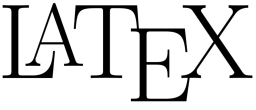
\includegraphics[opts]{img/logo}$.
You don't need to give the extension.

In this document, there are also macros defined for including images.
\begin{itemize}
\item \texttt{includeimage} includes an image from the image directory and
	centers it on the page
\item \texttt{includeimagefigure} same as include image but it does include it
	as a figure, a caption should be given and a label for the image will be set
\end{itemize}

\includeimagefigure[width=3cm,height=3cm][H][Logo]{logo}{Logo image of \LaTeX{}}
Logo image figure is \ref{img:logo}.

\subsubsection{TikZ}

TikZ\footnote{%
TikZ examples: \url{http://www.texample.net/tikz/examples/}}
is a library for drawing images directly in \LaTeX{}.
\begin{center}
\tikzstyle{block} = [rectangle, draw, fill=blue!20,
	text width=5em, text centered, rounded corners, minimum height=4em]
\tikzstyle{line} = [draw, -latex']
\begin{tikzpicture}
\node [block] (init) {initialize model};
\node [block, below of=init, node distance=6em] (stop) {stop};
\path [line] (init) -- (stop);
\end{tikzpicture}
\end{center}

There is also a library for writing plots \texttt{pgfplots}\footnote{%
PGF Plots examples: \url{http://www.texample.net/tikz/examples/pgfplots/}}.
\begin{center}
\begin{tikzpicture}
\begin{axis}
\addplot+[sharp plot] coordinates
{(0,0) (1,2) (2,3)};
\end{axis}
\end{tikzpicture}
\end{center}

\subsection{Code}

The \texttt{listings} package\footnote{%
Listings manual:
\url{http://mirror.ctan.org/macros/latex/contrib/listings/listings.pdf}}
is a powerful package for including code samples.

Code can be inserted using \texttt{lstlisting} environment, \texttt{lstinline}
command for a short code or \texttt{lstinputlisting} to read from a file.

\begin{lstlisting}[style=python]
# euh...
class Hello:
	"""
	does something
	"""
	def __init__(boom):
		print(1 + "hello world")
def main():
	bla = lambda x : x + 1
\end{lstlisting}

Writing abstract algorithms can be done using \texttt{algorithmicx} and
\texttt{algpseudocode} package.
An example is the algorithm \ref{alg:example}.

\begin{algorithm}[H]
\begin{algorithmic}[1]
\Require precondition
\Ensure postcondition
\State $y \leftarrow 1$
	\Comment{a comment}
\For{$i = 1 \to 10$} 
	\State $i \gets i + 1$
\EndFor
\While{condition}
	\State things
\EndWhile
\Repeat
	\State something
\Until{condition}
\Loop
	\State $i \leftarrow \infty$
\EndLoop
\end{algorithmic}
\caption{An example}
\label{alg:example}
\end{algorithm}


\vspace*{\fill}
%%%%%%%%%%
% Ending %
%%%%%%%%%%
%\clearpage

%% Bibliography, indexes and lists
%\listoffigures
%\listoftables
%\nocite{*} % include all citations
\printbibliography
\printindex
\vspace*{\fill}

%%%%%%%%%%%%
% Appendix %
%%%%%%%%%%%%
\appendix

%\input{appendix}

\end{document}
$.
In \LaTeX{} you don't need to specify the extension of included files.

\subsection{Environments}

You can create lists, enumerations, ...

\begin{itemize}
\item itemize
\item nested
	\begin{itemize}
	\item n
	\end{itemize}
\end{itemize}

\begin{enumerate}
\item enumerate
\item nested
	\begin{enumerate}
	\item n
	\end{enumerate}
\end{enumerate}

\begin{description}
\item[a] \emph{description}.
\item[b] something else
\end{description}

\begin{quote}
A simple quote.
\end{quote}

\begin{quotation}
A longer quotation.
\end{quotation}

\subsection{Text formatting}

\paragraph{Size}
You can change the size: {\tiny tiny}, {\scriptsize scriptsize}, {\footnotesize
footnotesize}, {\small small}, {\normalsize normal}, {\large large}, {\Large
Large}, {\LARGE LARGE}, {\huge huge} or {\Huge Huge}.

\paragraph{Font family}
You can use either \lstinline${\_family text}$ or \lstinline$\text_{text}$ where
\_ is: \textrm{rm}, \textsf{sf}, \texttt{tt}.

\paragraph{Series, shapes and related}
\begin{itemize}
\item \emph{emphasis}
\item {\bfseries bfseries} bold
\item {\mdseries mdseries} medium
\item {\upshape upshape} normal shape
\item {\itshape itshape} italic
\item {\scshape scshape} small capitals
\item {\slshape slshape} slanted \pcomment{oblique}
\end{itemize}

\paragraph{Colors}
The \texttt{xcolor} package allows you to write {\color{red} in red}.

\paragraph{Case-changing}
\uppercase{UpperCase \pagename}, \lowercase{LowerCase \pagename},
\MakeUppercase{MakeUppercase \pagename}, \MakeLowercase{MakeLowercase \pagename}.

\subsection{Spaces and boxes}
\footnote{\url{http://www.personal.ceu.hu/tex/spacebox.htm}}
First, let's describe some spacing commands:
\begin{itemize}
\item \lstinline$\vspace{length}$ verical space
\item \lstinline$\hspace{length}$ horizontal space \hspace{2cm} after 2cm
\item \lstinline$\hfill$ horizontal fill
\item \lstinline$\vspace*{\fill}$ dynamically sized vertical space
\end{itemize}

There are several boxes:
\mbox{mbox is a simple box},
\fbox{fbox is a box with a frame},
\parbox{2cm}{parbox has a fixed width},
\raisebox{2mm}{raisebox}.
\marginpar{marginpar gets here}
These are two rules:
\rule{5mm}{2mm}
\hfill \\
\rule{\linewidth}{0.3mm}

\paragraph{Minipage}
The minipage environment is similar to \lstinline$\parbox$ but it renders a page
instead of a box.

\begin{minipage}[b]{0.5\linewidth}
\begin{lstlisting}
\begin{minipage}[position]{width}
text
\end{minipage}
\end{lstlisting}
\end{minipage}

\subsection{Paragraph formatting}
\begin{center}
center or \lstinline$\centering$
\end{center}
\begin{flushright}
flushright or \lstinline$\raggedleft$
\end{flushright}
\begin{flushleft}
flushleft or \lstinline$\raggedright$
\end{flushleft}

\paragraph{Footnotes}
A footnote can be added using \lstinline!\footnote{}! which produces
\footnote{this}.

\section{Maths}

There are some environments for math formulae.

\paragraph{Text mode}
Included using \lstinline!$...$! or \lstinline$\( ... \)$.
You can use also \lstinline$\textstyle$ inside a formula.

\paragraph{Displayed mode}
Included using \lstinline$\[ ... \]$.
A displayed formula is centered on the page.
You can use also \lstinline$\displaystyle$ inside a formula.

\paragraph{Explicit mode}
Text: $\textstyle \sum_i$ - Diplayed: $\displaystyle \sum_i$

\subsection*{Some examples}
\[ \forall x \in X: \sum_{\alpha \in A} \frac{x^2}{\alpha + 1} \leq 1 \]
\[ A \overset{\textrm{def}}{=} (\Sigma, Q, Q_0, \delta) \]
\[ z = \overbrace{
	\underbrace{x}_\text{real} +
	\underbrace{iy}_\text{imaginary}
	}^\text{complex number}
\]
\[ A \xleftarrow{\text{this way}} B
	\xrightarrow[\text{or that way}]{} C \]
\begin{align*}
f(a, b)
	&= (a \vee b) \wedge a \\
	&= a
\end{align*}
\begin{equation}
\label{eq:matrix}
\begin{pmatrix}
1 & 0 & \cdots \\
0 & 1 & \ddots \\
\vdots & \ddots & \ddots \\
\end{pmatrix}
= (M_{i,j}) = \left\lbrace\begin{array}{cl}
1 & \quad \text{if $i = j$} \\
0 & \quad \text{otherwise} \\
\end{array}\right.
\end{equation}
There is a matrix in the equation \eqref{eq:matrix}.

\section{Extending \LaTeX{} - commands}

New commands and macros are always helpful to speed up writing and to have an
uniform layout.
A new command can be defined using \lstinline$\def$ or \lstinline$\newcommand$.

\begin{figure}[H]
\centering
\begin{minipage}{0.5\linewidth}
% source
\begin{lstlisting}[basicstyle=\scriptsize\ttfamily]
\def\hello<#1>{hello #1}
\newcommand{\helloworld}[2][comment]{%
\hello<#2 \pcomment{#1}>}
\newenvironment{king}
{\rule{1ex}{1ex}\hspace{\stretch{1}}}
{\hspace{\stretch{1}}\rule{1ex}{1ex}}

\helloworld{world}
\helloworld[invalid message]{nobody}

\begin{king}
My humble subjects...
\end{king}
\end{lstlisting}
\end{minipage}
\begin{minipage}{0.4\linewidth}
% result
\def\hello<#1>{hello #1}
\newcommand{\helloworld}[2][comment]{%
\hello<#2 \pcomment{#1}>}
\newenvironment{king}
{\rule{1ex}{1ex}\hspace{\stretch{1}}}
{\hspace{\stretch{1}}\rule{1ex}{1ex}}

\helloworld{world}
\helloworld[invalid message]{nobody}

\begin{king}
My humble subjects...
\end{king}
% end result
\end{minipage}
\caption{Example of command definition}
\end{figure}

\paragraph{Redeclaration}
\lstinline$\newcommand$ and \lstinline$\newenvironment$ issues an error when the
function already exists.
There exists also macros for re-declaring commands and environments:
\lstinline$\renewcommand$ and \lstinline$\renewenvironment$.

\subsection*{Other packages}
\begin{itemize}
\item \texttt{ifthen}: conditional compilation
\item \texttt{keyval}: key-value parameters
\item \texttt{optparams}: multiple optional parameters
\end{itemize}

\section{References}
\label{sec:ref}

References are links to declared labels on numbered elements \pcomment{such as
sections, figures, ...}.
Labels can be declared anywhere in the document using \lstinline$\label{name}$.
The \texttt{name} has often a prefix to differentiate referenced elements.

Then a reference can be included using:
\begin{itemize}
\item \texttt{ref} - \ref{sec:ref}
\item \texttt{nameref} - \nameref{sec:ref}
\item \texttt{pageref} - \pageref{sec:ref}
\item \texttt{autoref} - \autoref{sec:ref}
\item \texttt{shortref} (macro) - \shortref{sec:ref}
\item \texttt{textref} (macro) - \textref{sec:ref}{some text}
\end{itemize}

\subsection{Counters}

Counters are used to declare any numbers present in the document.

We can declare new counters or use existing ones.
A counter has a value (which is not directly printable), it is reset when the
parent has been incremented; also it can be used for references.
\begin{lstlisting}{style=latex}
\newcounter{name}[parent] % declares a new counter
\setcounter{name}{value} % sets the value
\addtocounter{name}{value} % adds a value
\stepcounter{name} % increments
\refstepcounter{name} % increments and is used by labels
\usecounter{name} % usage
\end{lstlisting}

\begin{table}[H]
\centering
\begin{tabular}{|c|c|}\hline
Command & Output \\ \hline
\lstinline!\alph{}! & \alph{section} \\
\lstinline!\Alph{}! & \Alph{section} \\
\lstinline!\arabic{}! & \arabic{section} \\
\lstinline!\roman{}! & \roman{section} \\
\lstinline!\Roman{}! & \Roman{section} \\
\hline
\end{tabular}
\caption{Rendering of the counter named \texttt{section}}
\end{table}

\subsection{Theorems}

Theorems in \LaTeX are more general than simpe theorems in maths.
There is an environment for declaring "types of theorems".
This is done in the preamble of the document.
\begin{lstlisting}
\newtheorem{name}[counter]{text}[section]
\end{lstlisting}
This command declares a theorem type named \texttt{name} using a named counter
which is reset at every section, subsection, etc.
There also is \lstinline!\newtherem*! does not use any counters.
\texttt{text} defines here what should be printed in the document as the type of
the theorem.

This document (and also Beamer) defines some theorem types such as
\textit{lemma}, \textit{theorem}, \textit{definition}, ...
Also, \lstinline!\theoremstyle! can be used to declare new formatting for
theorems; the predefined formattings are \textit{plain}, \textit{definition} and
\textit{remark}.

\begin{definition}
Some standard definition.
\end{definition}

\begin{theorem}
My theorem...
\end{theorem}
\begin{theorem}
Another theorem...
\begin{proof}
This is the \emph{proof} environment...
\end{proof}
\end{theorem}

\newtheorem{mydef}{$\Rightarrow$ DEF}
\begin{mydef}
mydef usage declared as \lstinline!\newtheorem{mydef}{$\Rightarrow$ DEF}!.
\end{mydef}

\section{Figures}

Floating elements are things that cannot be broken between two pages.
Most often they are figures and tables.
Captions and labels may be attached to figures.

\begin{figure}[H]
\centering
\begin{lstlisting}
\begin{figure}[placement]
body
\caption{caption of the figure}
\label{label}
\end{figure}
\end{lstlisting}
\caption{Figure placement}
\label{fig:figure-placement}
\end{figure}

Placement is:
\begin{itemize}
\item H: here
\item t: top of the page
\item b: bottom of the page
\item p: put on a special page for figures
\end{itemize}

\subsection{Tables}

For tables, they are included in the same way as figures, the environment name
is \texttt{table}.
Then the body of a text may contain a tabular environment, most common are:
\texttt{tabular}, \texttt{tabularx} and \texttt{array}.

\begin{table}[H]
\centering
\begin{tabular}{l|c|r}
\hline\hline
left & center & right \\
\hline
\hspace{2cm} & \hspace{2cm} & \hspace{2cm} \\
\end{tabular}
\caption{\texttt{tabular} environment}
\end{table}

\begin{table}[H]
\centering
\begin{tabularx}{0.8\linewidth}{|c|>{\centering $before-}X<{-after$}|p{1cm}|}
centered & rest & 1cm \\
\end{tabularx}
\caption{\texttt{tabularx} environment}
\end{table}

Other commands exist for column spanning:
\begin{itemize}
\item \lstinline$\multicolumn{num_cols}{alignment}{contents}$
\item \lstinline$\multirow{num_rows}{width}{contents}$
\end{itemize}

\subsection{Images}

\subsubsection{Including}

Including images can be done using \lstinline$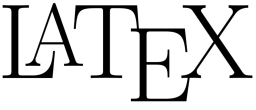
\includegraphics[opts]{img/logo}$.
You don't need to give the extension.

In this document, there are also macros defined for including images.
\begin{itemize}
\item \texttt{includeimage} includes an image from the image directory and
	centers it on the page
\item \texttt{includeimagefigure} same as include image but it does include it
	as a figure, a caption should be given and a label for the image will be set
\end{itemize}

\includeimagefigure[width=3cm,height=3cm][H][Logo]{logo}{Logo image of \LaTeX{}}
Logo image figure is \ref{img:logo}.

\subsubsection{TikZ}

TikZ\footnote{%
TikZ examples: \url{http://www.texample.net/tikz/examples/}}
is a library for drawing images directly in \LaTeX{}.
\begin{center}
\tikzstyle{block} = [rectangle, draw, fill=blue!20,
	text width=5em, text centered, rounded corners, minimum height=4em]
\tikzstyle{line} = [draw, -latex']
\begin{tikzpicture}
\node [block] (init) {initialize model};
\node [block, below of=init, node distance=6em] (stop) {stop};
\path [line] (init) -- (stop);
\end{tikzpicture}
\end{center}

There is also a library for writing plots \texttt{pgfplots}\footnote{%
PGF Plots examples: \url{http://www.texample.net/tikz/examples/pgfplots/}}.
\begin{center}
\begin{tikzpicture}
\begin{axis}
\addplot+[sharp plot] coordinates
{(0,0) (1,2) (2,3)};
\end{axis}
\end{tikzpicture}
\end{center}

\subsection{Code}

The \texttt{listings} package\footnote{%
Listings manual:
\url{http://mirror.ctan.org/macros/latex/contrib/listings/listings.pdf}}
is a powerful package for including code samples.

Code can be inserted using \texttt{lstlisting} environment, \texttt{lstinline}
command for a short code or \texttt{lstinputlisting} to read from a file.

\begin{lstlisting}[style=python]
# euh...
class Hello:
	"""
	does something
	"""
	def __init__(boom):
		print(1 + "hello world")
def main():
	bla = lambda x : x + 1
\end{lstlisting}

Writing abstract algorithms can be done using \texttt{algorithmicx} and
\texttt{algpseudocode} package.
An example is the algorithm \ref{alg:example}.

\begin{algorithm}[H]
\begin{algorithmic}[1]
\Require precondition
\Ensure postcondition
\State $y \leftarrow 1$
	\Comment{a comment}
\For{$i = 1 \to 10$} 
	\State $i \gets i + 1$
\EndFor
\While{condition}
	\State things
\EndWhile
\Repeat
	\State something
\Until{condition}
\Loop
	\State $i \leftarrow \infty$
\EndLoop
\end{algorithmic}
\caption{An example}
\label{alg:example}
\end{algorithm}

\section{Bibliography}

Getting the bibliography at the end of the document usually isn't an easy nor
fascinating task to do.
Hopefully, \LaTeX{} has a very good support for it using \texttt{bibtex} and
optionally a package named
\texttt{biblatex}\footnote{\url{http://ctan.org/tex-archive/macros/latex/exptl/biblatex/doc/biblatex.pdf}}.

Your bibliography is declared in a separate file with an extension
\texttt{.bib}, it is parsed and \emph{cited} references are automatically added
to the end of the document.
They are properly formatted and even sorted.

To cite an entry, use \lstinline!\cite{name}!.
For example, \citetitle{latex-comprehensive-symbol} is
\cite{latex-comprehensive-symbol}.
There is also an alternative version: \lstinline!\nocite{name}!;
it will not print anything but the reference will still appear at the end of the
document.
A special name \texttt{*} can be used to cite everything.
